\documentclass[11pt]{beamer}
\usepackage{subfig}
\usepackage{graphicx} 
\usepackage{caption}
\usepackage{beamerthemePadova}
\usepackage{amsmath}
\usepackage{hyperref}
\usepackage{graphicx}
\usepackage{multirow}
\usepackage{tikz}

\usepackage[utf8]{inputenc}
\usepackage[T1]{fontenc}
\usepackage{mathtools}
\usepackage{lmodern}
\usepackage{textcomp}
\captionsetup[figure]{labelformat=empty}

\title[Hierarchical Healthcare Facility Location]{Hierarchical Healthcare Facility Location}
\author[Daniele Bugatti \& Giovanni Gaio]{Daniele Bugatti \and Giovanni Gaio}
\date{\today}

\begin{document}

% Title (slide 1)
\begin{frame}[plain]
  \titlepage
\end{frame}
% Idea (slide 2)
\section{Idea}
\begin{frame}{The Idea --- What we do}
  \begin{itemize}
    \item \textbf{Integrated Network Design:} Strategically placing healthcare facilities where high-level hubs and local clinics are co-located to minimize infrastructure costs. 
    
    \item \textbf{Graph-Based Optimization:} Modeling the region as a weighted graph—where nodes represent urban centers weighted by population—to determine the optimal placement of Tier-1 and Tier-2 facilities for maximum coverage.
  \end{itemize}

  \vfill

  \begin{center}
    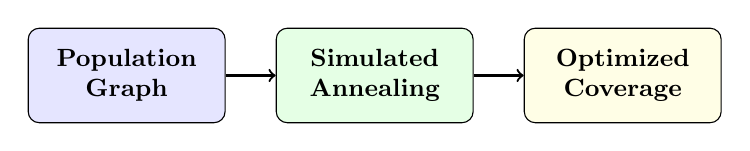
\begin{tikzpicture}[
      scale=0.9,
      box/.style={draw, rounded corners, fill=#1, align=center, minimum width=2.5cm, minimum height=1.2cm, font=\small\bfseries}
    ]
      \node[box=blue!10] (A) at (0,0) {Population \\ Graph};
      \node[box=green!10] (B) at (3.5,0) {Simulated \\ Annealing};
      \node[box=yellow!10] (C) at (7,0) {Optimized \\ Coverage};
      
      \draw[->, thick] (A) -- (B);
      \draw[->, thick] (B) -- (C);
    \end{tikzpicture}
  \end{center}
  
  \vfill
  % {\tiny Presenter note: ~60s. Focus on the transition from demographic data to spatial optimization via SA.}
\end{frame}

% Usefulness (slide 3)

\section{Usefulness}
\begin{frame}{Who Benefits \& Why It Matters}
  \begin{itemize}
    \item A \textbf{Decision Support System} for shifting from fragmented local development to a \textbf{coordinated strategic framework}.
    \begin{itemize}
        \item \textit{Emerging Contexts:} Designing optimized networks from the ground up.
        \item \textit{Legacy Contexts:} Rationalizing and reallocating hubs in over-saturated or inefficient areas.
    \end{itemize}

    \vfill

    \item We exploit \textbf{economies of scope} through hierarchical nesting to minimize infrastructure costs, enabling \textbf{co-location savings}.
    \begin{itemize}
        \item A generalizable framework applicable to any service network requiring tiered distribution (e.g., logistics, retail, or emergency services).
    \end{itemize}
  \end{itemize}
  \vfill
\end{frame}

% Problem Formalization (slide 4)
\section{Problem Formalization}
\begin{frame}{Problem Formalization \& Search Space}
  
  % Box con la formalizzazione
  \begin{block}{The Hierarchical Facility Location Problem (HFLP)}
    \begin{itemize}
        \item \textbf{Input:} A weighted graph $G=(V, E)$, where $w_i$ represents the population of node $i$, and the number of facilities to be placed for each level ($k_1, k_2$).
        \item \textbf{Output:} An optimal allocation of facilities $S_1, S_2 \subset V$, such that $|S_l| = k_l$ and $S_2 \subseteq S_1$ (\textbf{Nested Hierarchy})
        \item \textbf{Objective:} Minimize $Z = \sum_{l \in Levels} \alpha_l \cdot \Phi_j$, where $\Phi_j$ is a distance-based function to the nearest facility of level $j$.
    \end{itemize}
  \end{block}

  \vfill

  \begin{itemize}
    \item The HFLP is Search Problem where the search space
    $\mathcal{S}$ is composed by all possible permutation of facility locations. 
  \end{itemize}
  \[
  |\mathcal{S}| = \binom{|V|}{k_1} \binom{k_1}{k_2}
  \]
  \vfill
\end{frame}

% Simulated Annealing (slide 5)
\section{Our Approach}
\begin{frame}{Solving with Simulated Annealing}
  \begin{itemize}
    \item Exact solvers (ILP) are computationally infeasible for large-scale networks due to the \textbf{combinatorial explosion} of the search space.
    \end{itemize}
  \vfill

  \begin{block}{Simulated Annealing}
    \begin{itemize}
      \item \textbf{Neighborhood:} Relocation of one facility, maintaining the nested constraint ($S_2 \subseteq S_1$)
      \item \textbf{Temperature Schedule:} $T_{i+1} = \alpha T_{i}, \ 0<\alpha<1$
      \item \textbf{Acceptance Probability:}
      \[ 
      P(S \to S') = 
      \begin{cases} 
      1 & \text{if } \Delta Z < 0 \\
      e^{-\frac{\Delta Z}{T}} & \text{if } \Delta Z \geq 0 
      \end{cases}
      \]
    \end{itemize}
  \end{block}

  \vfill
\end{frame}


\section{Outcome}
\begin{frame}{Performance \& Validation}
  \begin{itemize}
    \item \textbf{Goal:} We aim to obtain near-optimal solutions in polynomial time, avoiding the exponential explosion of exact ILP solvers.
    \vspace{10pt}

    \item \textbf{Validation:} Benchmarking on small synthetic networks, for which an exact solution is computable, to verify a negligible optimality gap.

    \vfill

    \item \textbf{Veneto Case Study:} We will apply our solver to the regional healthcare network to compare the optimized model with the current actual distribution.
  \end{itemize}
\end{frame}

% Closing / questions (slide 6)
\begin{frame}{Conclusion \& Questions}
  \begin{itemize}
    \item \textbf{Summary:} We developed a \textbf{Simulated Annealing} solver to optimize \textbf{hierarchical healthcare networks}, balancing citizen accessibility and infrastructure costs on a regional scale (\textit{Veneto case study}).
  \end{itemize}
\end{frame}
\begin{frame}
  \begin{center}
    Questions?\\{\tiny Contacts: \texttt{giovanni.gaio.1@studenti.unipd.it} \;|\; \texttt{daniele.bugatti@studenti.unidpd.it}}
  \end{center}
\end{frame}

\end{document}
